\documentclass[10pt, aspectratio=169]{beamer}

% Tema e Cores
\usetheme{Madrid}
\usecolortheme{default}

% Pacotes de Idioma, Codificação e Gráficos
\usepackage[utf8]{inputenc}
\usepackage[T1]{fontenc}
\usepackage[brazilian]{babel}
\usepackage{amsmath, amssymb}
\usepackage{booktabs}
\usepackage{multirow}
\usepackage{graphicx}
\usepackage{adjustbox}
\usepackage{caption}
\usepackage{fontawesome5}

% Pacotes para os Diagramas (TikZ)
\usepackage{tikz}
\usetikzlibrary{calc, positioning, shapes.geometric, arrows.meta, fit, backgrounds}

% Configurações de Título
\title[Dashboard Analítico em R]{Dashboard Analítico em R para Visualização Interativa, Modelagem Temporal e Relatórios Parametrizados}

\author[Valente, Silva, Salim, Oliveira]{\textbf{Gabriel Baia da Silva}\inst{2} \and \textbf{Mário Diego Rocha Valente}\inst{1,2} \\ \and \textbf{Kleber Bezerra Salim}\inst{2} \and \textbf{Tito Félix de Oliveira}\inst{2}}

\institute[DETRAN-PA \& UFPA]{
  \inst{1} Faculdade de Computação -- Universidade Federal do Pará (UFPA) \and
  \inst{2} Departamento de Trânsito do Estado do Pará (DETRAN-PA) 
}

\date{Defesa de Artigo}

\begin{document}

% --- SLIDE 1: Capa ---
\begin{frame}
    \titlepage
\end{frame}

% --- SLIDE 2: Sumário ---
\begin{frame}{Roteiro da Apresentação}
    \tableofcontents
\end{frame}

% ==========================================
% SEÇÃO 1: INTRODUÇÃO E OBJETIVOS
% ==========================================
\section{Contextualização e Objetivos}

\begin{frame}{Contextualização}
    \begin{itemize}
        \item \textbf{Cenário Atual:} O crescimento da produção de dados governamentais exige mecanismos eficazes de transparência pública e apoio à tomada de decisão.
        \item \textbf{O Desafio:} Órgãos executivos de trânsito demandam soluções computacionais que unam processamento estatístico, visualização interativa e relatórios automatizados, superando o modelo de atendimento manual de solicitações.
        \item \textbf{Limitações Tradicionais:} As ferramentas proprietárias de \textit{Business Intelligence} (BI) frequentemente esbarram em altos custos, dependência de fornecedor (\textit{vendor lock-in}) e algoritmos \textit{black-box}.
    \end{itemize}
\end{frame}

\begin{frame}{Natureza dos dados}
    \begin{block}{A Origem dos Dados}
        Os dados processados no dashboard são obtidos a partir do banco de dados interno do DETRAN PA, sob requisição semestral.
    \end{block}
    
    \vspace{0.3cm}
    \textbf{Características Estatísticas:}
    \begin{itemize}
        \item 144 localidades, observações mensais.
        \item Quantidade de veículos Veículos observada por categoria e agrupada por mês. 
        \item Base com variáveis numéricas, categóricas e temporais (mista).
        \item Meses configurados como variáveis cíclicas a cada ano, nos dando capacidade de observação sazonal.
    \end{itemize}
\end{frame}

\begin{frame}{Objetivos do Estudo}
    \begin{block}{Objetivo Principal}
        Desenvolver uma arquitetura analítica integrada para disponibilização pública de estatísticas da frota veicular, utilizando tecnologias \textit{open-source}.
    \end{block}
    
    \vspace{0.3cm}
    \textbf{Objetivos Específicos:}
    \begin{itemize}
        \item Integrar processamento \textit{lazy-loading} colunar com \textbf{Apache Arrow}.
        \item Criar painéis interativos com o \textit{framework} \textbf{Shiny} e relatórios paramétricos via \textbf{Quarto}.
        \item Projetar o crescimento da frota até 2031 comparando modelos estatísticos (SARIMAX) e de Aprendizado Profundo (LSTM e GRU).
        \item Assegurar alta disponibilidade através de um fluxo \textbf{DevOps} (Kubernetes).
    \end{itemize}
\end{frame}

% ==========================================
% SEÇÃO 2: ARQUITETURA E TECNOLOGIAS
% ==========================================
\section{Arquitetura e Metodologia}

\begin{frame}{Arquitetura do Sistema}
    \begin{figure}[H]
        \centering
        \resizebox{0.8\textwidth}{!}{%
        \begin{tikzpicture}[
            node distance=0.5cm and 1.6cm,
            box/.style={draw, rounded corners = 3pt, rectangle, minimum width=2.5cm, minimum height=0.85cm, align=center, font=\small},
            db/.style={draw, cylinder, shape border rotate=90, aspect=0.25, minimum width=2.5cm, minimum height=0.85cm, align=center, font=\small},
            arrow/.style={-Stealth, thick}, 
            barrow/.style={Stealth-Stealth, thick}
        ]
        %% COLUNA 1
        \node[db] (A) {\Large\faDatabase\\[4pt] Fontes de Dados\\{\footnotesize (.csv/.xls)}};
        \node[box, below=of A] (B) {\Large\faCogs\\[4pt] Processamento ETL\\{\footnotesize (\textit{Tidyverse})}};
        \node[db,  below=of B] (C) {\Large\faBolt\\[4pt] Dados Otimizados\\{\footnotesize (\textit{Arrow / Parquet})}};
        \draw[arrow] (A) -- (B);
        \draw[arrow] (B) -- (C);
        \begin{scope}[on background layer]
          \node[draw, dashed, inner sep=0.3cm, fit=(A)(B)(C), label={[font=\footnotesize]above:Preparação de Dados}] (box1) {};
        \end{scope}

        %% COLUNA 2
        \node[box, right=1.8cm of B] (D) {\Large\faServer\\[4pt] Motor Reativo (dplyr)\\{\footnotesize Lógica do Servidor}};
        \node[box, above right=0.4cm and 1.2cm of D] (E) {\Large\faChartLine\\[4pt] Modelagem\\{\footnotesize ARIMA / GRU}};
        \node[box, right=1.2cm of D]                 (F) {\Large\faDesktop\\[4pt] Interface UI\\{\footnotesize bs4Dash}};
        \node[box, below right=0.4cm and 1.2cm of D] (G) {\Large\faChartBar\\[4pt] Visualizações\\{\footnotesize echarts4r / leaflet}};
        \draw[barrow] (D) -- (E);
        \draw[arrow] (D) -- (F);
        \draw[arrow] (D) -- (G);
        \begin{scope}[on background layer]
          \node[draw, dashed, inner sep=0.3cm, fit=(D)(E)(F)(G), label={[font=\footnotesize]above:Aplicação R -- Shiny}] (box2) {};
        \end{scope}

        %% COLUNA 3
        \node[box, right=1.2cm of F] (H) {\Large\faGlobe\\[4pt] Renderização\\{\footnotesize Navegador Web}};
        \node[db,  below=of H]       (I) {\Large\faCubes\\[4pt] Produção DevOps\\{\footnotesize \textit{Podman/Kubernetes}}};
        \begin{scope}[on background layer]
          \node[draw, dashed, inner sep=0.3cm, fit=(H)(I), label={[font=\footnotesize]above:Saída e Hospedagem}] (box3) {};
        \end{scope}

        %% CONEXÕES
        \draw[arrow] (C.east) -- ++(1,0) coordinate (ElbowLL) -- (D.west);
        \node[below=2pt, font=\scriptsize] at (ElbowLL) {Lazy Loading};
        \draw[arrow] (F) -- (H);
        \draw[arrow] (G) -- (H);
        \draw[arrow] (box2.south) -- ++(0,-1.4) -| node[below, font=\scriptsize, pos=0.25]{Pipeline CI/CD} (I.south);
        \end{tikzpicture}%
        }
        \caption{Fluxo de dados: do \textit{lazy-loading} colunar à implantação.}
    \end{figure}
\end{frame}

% ==========================================
% SEÇÃO 3: RESULTADOS - VISUALIZAÇÃO INTERATIVA
% ==========================================
\section{Telas do Dashboard}

\begin{frame}{Painel de Resumo Macroeconômico}
    \begin{figure}[H]
        \centering
        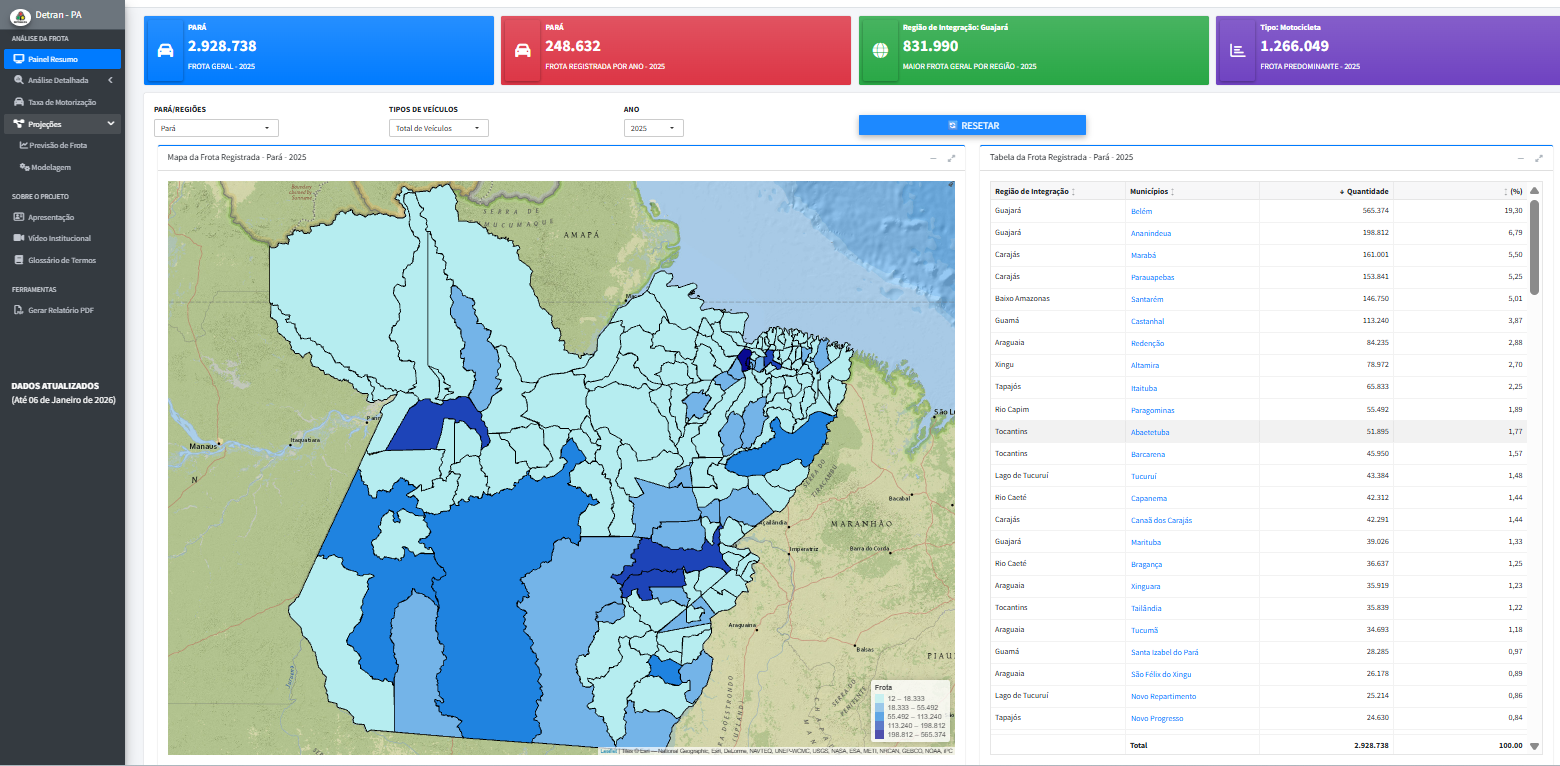
\includegraphics[width=\textwidth,height=0.75\textheight,keepaspectratio]{PainelResumo.png}
        \caption{Aba Principal do dashboard desenvolvido em Shiny..}
    \end{figure}
\end{frame}

\begin{frame}{Painel de Análise Detalhada}
    \begin{figure}[H]
        \centering
        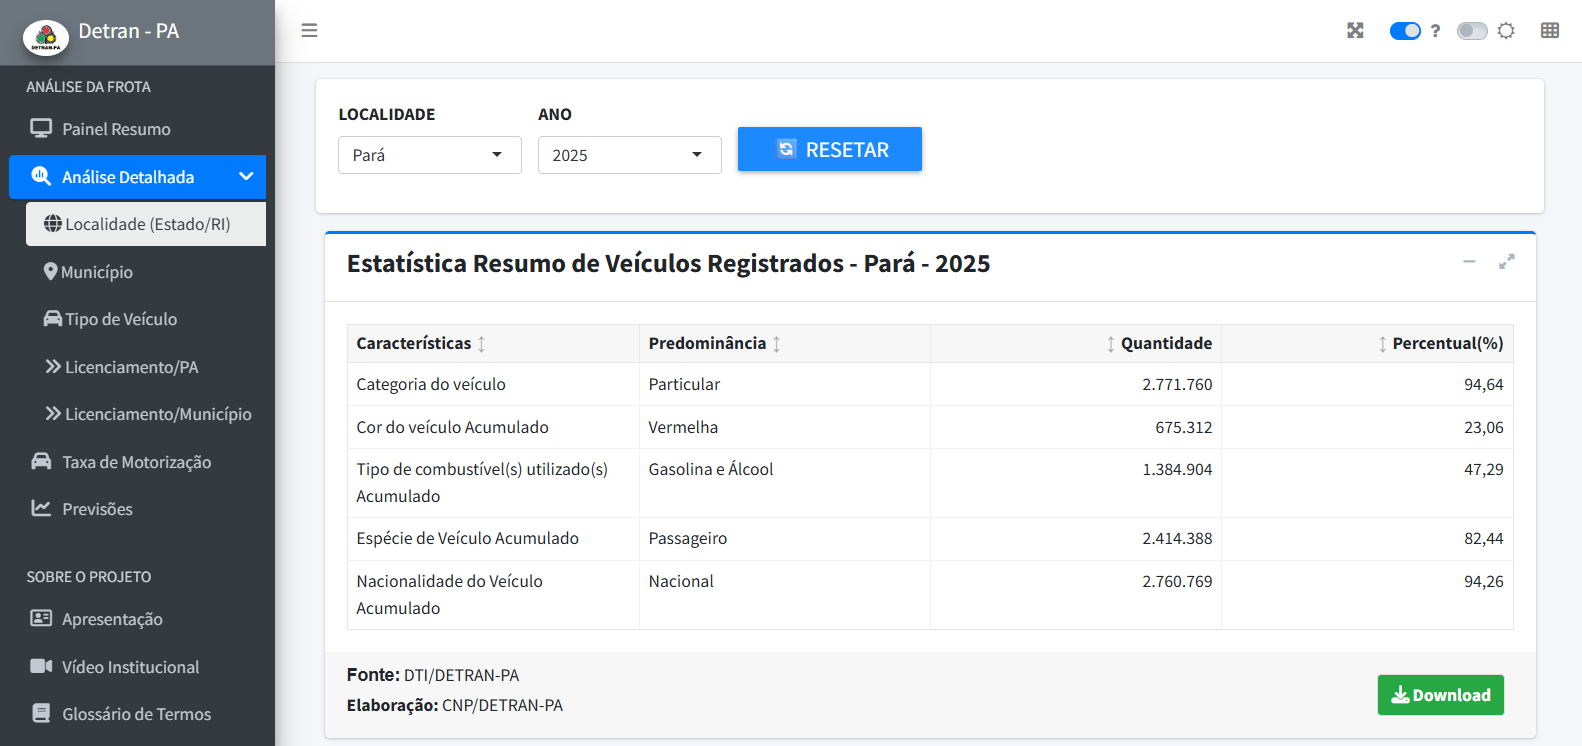
\includegraphics[width=\textwidth,height=0.75\textheight,keepaspectratio]{PainelDetalhes.png}
        \caption{Estatística Resumo sobre os Veículos Registrados}
    \end{figure}
\end{frame}

\begin{frame}{Painel de Taxa de Motorização}
    \begin{figure}[H]
        \centering
        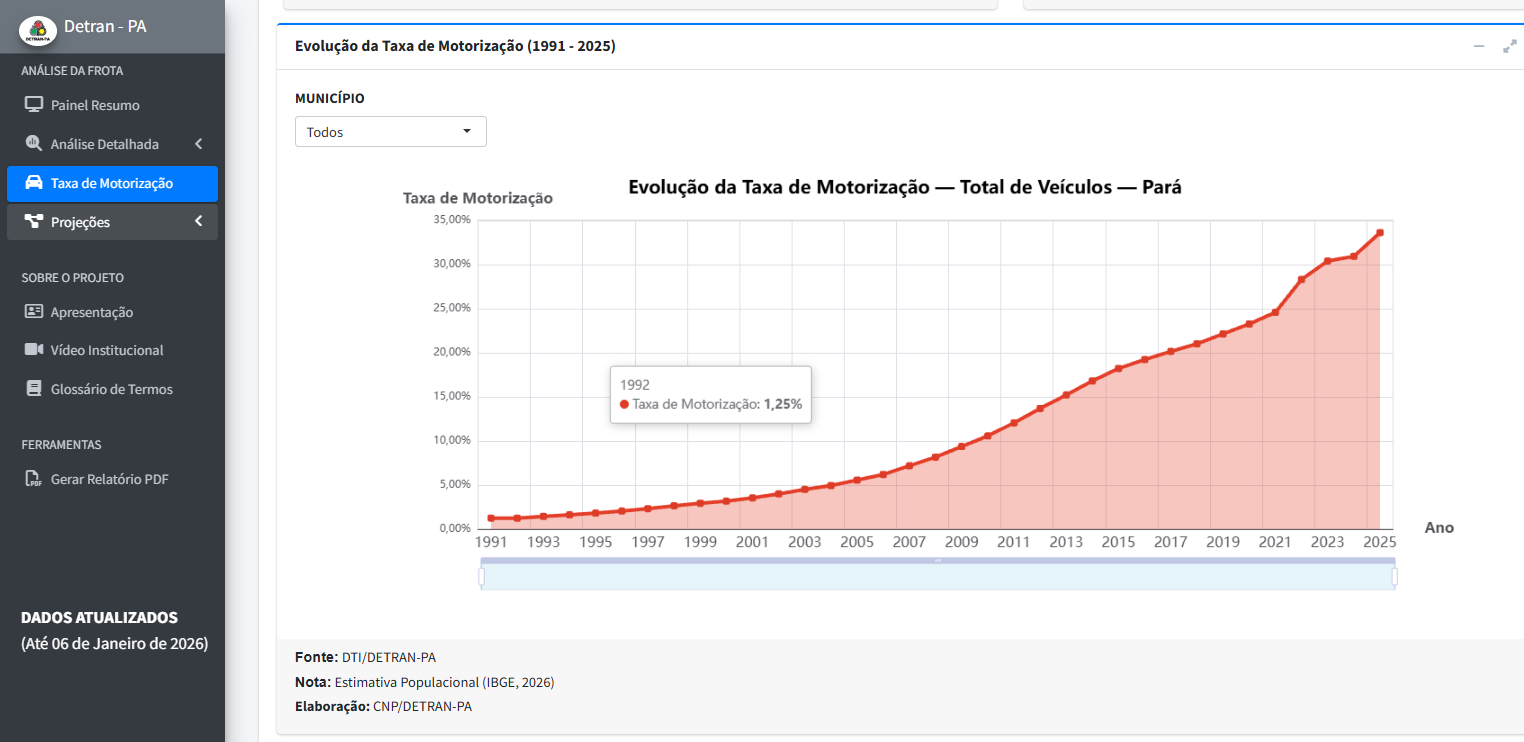
\includegraphics[width=\textwidth,height=0.75\textheight,keepaspectratio]{GraficoTaxaMotorizacao.png}
        \caption{Taxa de Motorização sobre os Veículos Registrados.}
    \end{figure}
\end{frame}

\begin{frame}{Painel de Previsão Analítica}
    \begin{figure}[H]
        \centering
        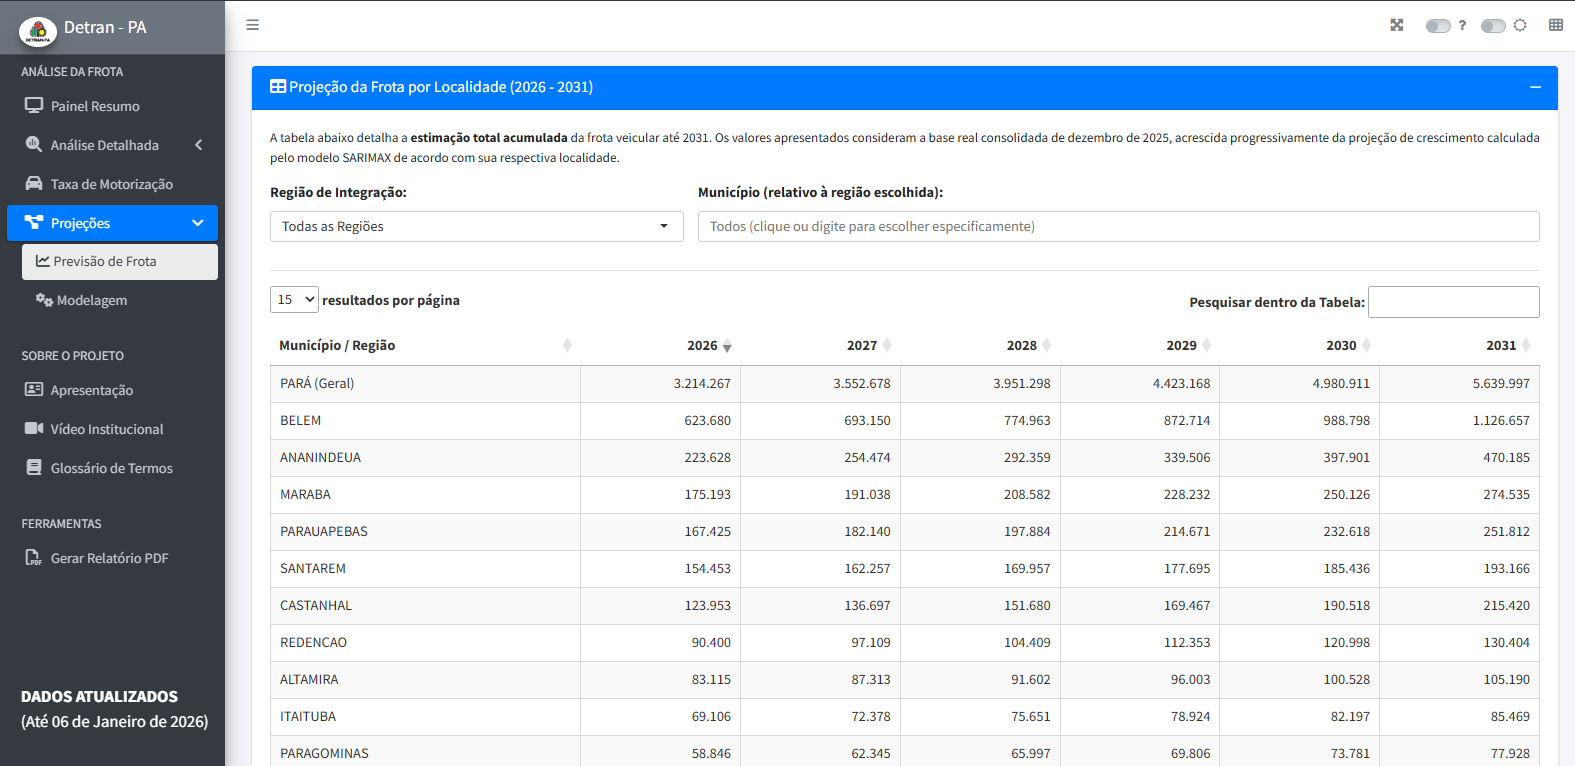
\includegraphics[width=\textwidth,height=0.75\textheight,keepaspectratio]{PainelPrevisoes.png}
        \caption{Painel de Previsões Temporais e Comparação de Modelos.}
    \end{figure}
\end{frame}

% ==========================================
% SEÇÃO 4: RESULTADOS - MODELAGEM
% ==========================================
\section{Resultados Preditivos}

\begin{frame}{Modelagem Estatística: Família ARIMA}
    \small
    \begin{block}{ARIMA $(p,d,q)$: dependência temporal e tendência}
        Combina autorregressão ($p$), diferenciação ($d$) e médias
        móveis dos erros ($q$) para modelar a evolução mensal da frota.
        A diferenciação trata a tendência da série.
    \end{block}

    \begin{block}{SARIMA $(p,d,q)(P,D,Q)_{12}$: sazonalidade anual}
        Acrescenta componentes autorregressivos, diferenciação e
        médias móveis sazonais ($P,D,Q$), com período de
        \textbf{12 meses}, associado ao calendário de IPVA e licenciamentos.
    \end{block}

    \begin{block}{SARIMAX: sazonalidade e intervenção econômica}
        Inclui regressores exógenos ($X_t$). No estudo, uma
        \textbf{intervenção de pulso} representou as retrações
        macroeconômicas brasileiras de \textbf{2013--2017},
        incorporando esse choque à modelagem da série.
    \end{block}

    \vspace{0.15cm}
    \footnotesize
    \textbf{Avaliação:} 12 meses finais reservados para teste.
    \quad \textbf{Projeções:} até 2031, pré-calculadas e carregadas no Shiny.
\end{frame}

\begin{frame}{Projeção Estatística Clássica: SARIMAX}
    \begin{figure}[H]
        \centering
        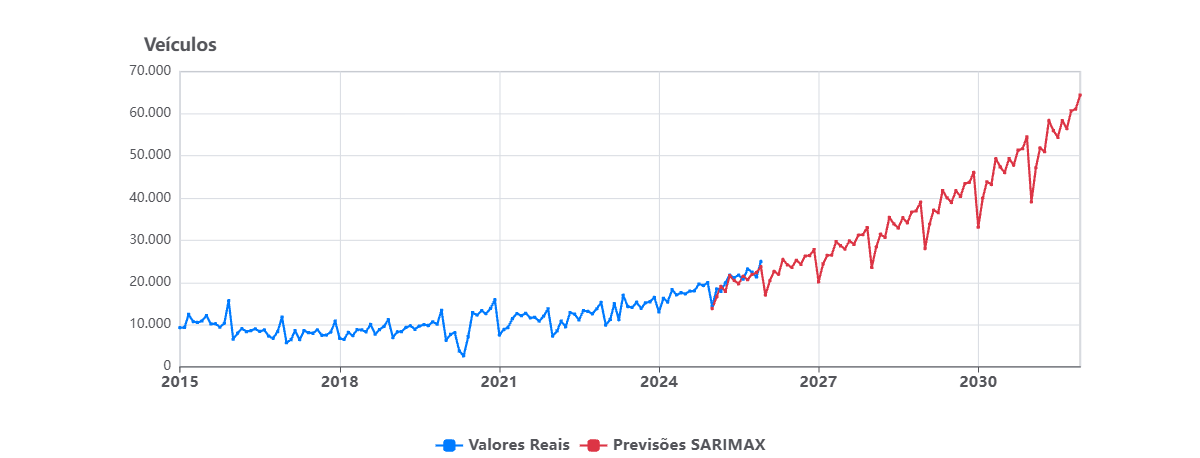
\includegraphics[width=\textwidth,height=1\textheight,keepaspectratio]{GraficoSarimax.png}
        \caption{Previsão estatística de crescimento obtida com o modelo SARIMAX.}
    \end{figure}
\end{frame}

\begin{frame}{Hiperparâmetros dos Modelos LSTM e GRU}
    \small
    \begin{table}[H]
        \centering
        \caption{Configurações de treinamento descritas no artigo.}
        \renewcommand{\arraystretch}{1.1}
        \begin{tabular*}{0.95\textwidth}{@{\extracolsep{\fill}}l|c|c@{}}
            \hline \hline
            \textbf{Parâmetro} & \textbf{LSTM} & \textbf{GRU} \\
            \hline \hline
            Escopo do modelo & Por localidade & Global \\
            Camadas e unidades
                & $\mathrm{LSTM}(32) \rightarrow \mathrm{Dense}(1)$
                & $\mathrm{GRU}(32) \rightarrow \mathrm{Dense}(1)$ \\
            Janela de entrada & 24 meses & 24 meses \\
            Otimizador & Adam & Adam \\
            Taxa de aprendizado & $0{,}01$ & $0{,}01$ \\
            Função de perda & MSE & MSE \\
            Número de épocas & 100 & 100 \\
            Tamanho do lote & 8 & 32 \\
            Validação interna & 10\% & 10\% \\
            Semente aleatória & 42 & 42 \\
           \hline \hline
        \end{tabular*}
    \end{table}

    \vspace{0.1cm}
    \footnotesize
    \textbf{Histórico:} 2016--2025.
    \quad \textbf{Teste temporal:} 12 meses finais da série.
\end{frame}



\begin{frame}{Projeção via Deep Learning: LSTM x GRU}
    \begin{figure}[H]
        \centering
        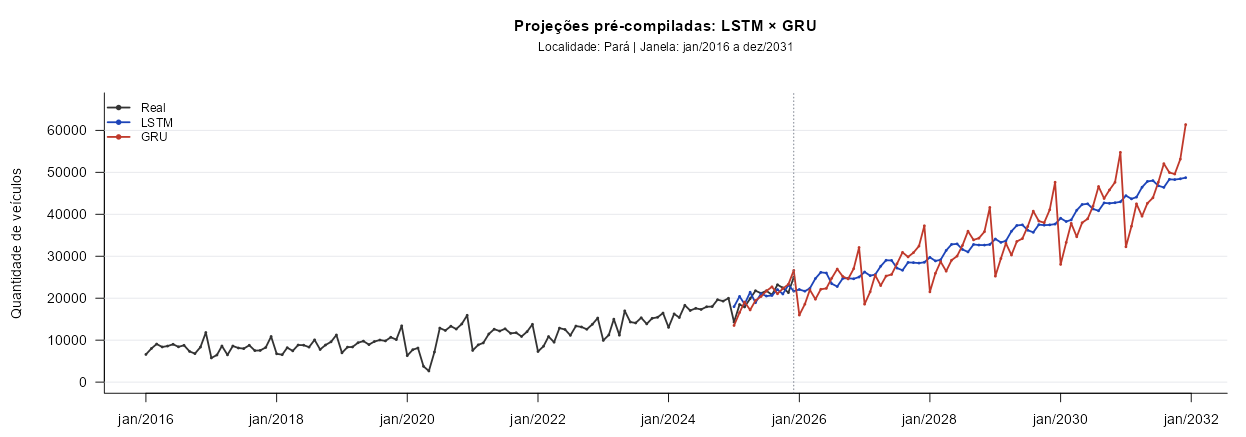
\includegraphics[width=\textwidth,height=1\textheight,keepaspectratio]{LSTMxGRU.png}
        \caption{Projeção dos algoritmos LSTM e GRU 2025-2031.}
    \end{figure}
\end{frame}

\begin{frame}{Abordagem Preditiva: O Tensor Multidimensional GRU}
    \begin{figure}[H]
        \centering
        \resizebox{0.8\textwidth}{!}{%
        \begin{tikzpicture}[
            node distance=1cm and 1.2cm,
            box/.style={draw, rectangle, rounded corners=4pt, minimum width=2.8cm, minimum height=1.5cm, align=center, font=\small},
            arrow/.style={-Stealth, thick, color=black!80}
        ]
        \node[box, fill=blue!10, draw=blue!40] (tensor) {\textbf{Tensor de Entrada 3D}\\ {\scriptsize (Modelagem de Dados)}\\[6pt] \footnotesize $[Amostras \times Passos \times Variáveis]$ \\ \footnotesize $(M \times 24 \times N)$};
        \node[box, right=of tensor, fill=green!10, draw=green!50] (gru) {\textbf{Camada GRU}\\ \footnotesize Extração de Padrões\\ \footnotesize Espaço-Temporais Ocultos};
        \node[box, right=of gru, fill=orange!10, draw=orange!50] (dense) {\textbf{Camada Densa}\\ \footnotesize Recombinação Linear\\ \footnotesize (Função de Ativação)};
        \node[box, right=of dense, fill=red!10, draw=red!40] (output) {\textbf{Vetor de Saída}\\ \footnotesize Previsão $t+h$};

        \draw[arrow] (tensor) -- node[above, font=\scriptsize] {\textit{Batching}} (gru);
        \draw[arrow] (gru) -- node[above, font=\scriptsize] {$H_{t}$} (dense);
        \draw[arrow] (dense) -- (output);
        \end{tikzpicture}%
        }
        \caption{Solução para esparsidade de dados: transferência de \textit{features} de grandes polos urbanos para mitigar escassez em cidades menores.}
    \end{figure}
\end{frame}

\begin{frame}{Métricas de Avaliação}
    \small
    As métricas foram calculadas sobre os 12 meses finais da série, reservados para o conjunto de teste.
    
    \vspace{0.25cm}
    \begin{columns}[T,onlytextwidth]
        \begin{column}{0.48\textwidth}
            \begin{block}{Erros de previsão}
                \begin{itemize}
                    \item \textbf{MAPE:} erro percentual médio absoluto. Facilita a interpretação relativa, mas é sensível a valores reais próximos de zero.
                    \item \textbf{MAE:} média dos erros absolutos. Indica, na unidade original, o erro médio cometido pelo modelo.
                    \item \textbf{RMSE:} raiz do erro quadrático médio. Penaliza mais fortemente erros grandes.
                \end{itemize}
            \end{block}
        \end{column}
        \begin{column}{0.48\textwidth}
            \begin{block}{Ajuste e parcimônia}
                \begin{itemize}
                    \item \textbf{$R^2$:} proporção da variabilidade dos dados explicada pelo modelo. Quanto maior, melhor o ajuste relativo.
                    \item \textbf{AIC:} combina qualidade do ajuste e complexidade do modelo. Valores menores favorecem modelos mais parcimoniosos.
                    \item \textbf{BIC:} critério semelhante ao AIC, com penalização maior para modelos mais complexos.
                \end{itemize}
            \end{block}
        \end{column}
    \end{columns}
    
    \vspace{0.2cm}
\end{frame}

\begin{frame}{Avaliação de Desempenho e Comparação de Modelos}
    Validação realizada sobre os 12 meses finais da série (\textit{Test-Set}):
    
    \vspace{0.5cm}
    \begin{table}[H]
        \centering
        \caption{Métricas de desempenho no conjunto de validação}
        \resizebox{0.9\textwidth}{!}{%
        \begin{tabular}{l|c|c|c|c|c|c}
        \hline \hline
        \textbf{Modelo} & \textbf{MAPE (\%)} & \textbf{MAE} & \textbf{RMSE} & \textbf{AIC} & \textbf{BIC} & \textbf{$R^2$} \\
        \hline \hline
        LSTM    & 9,07 & 1,803 & 2,292 & 189,70 & 190,67 & 0,2581 \\
        GRU     & \textbf{5,19} & \textbf{1,129} & 1,634 & 181,57 & 182,54 & 0,6230 \\
        ARIMA   & 9,18 & 1,855 & 2,203 & 188,74 & 189,71 & 0,3150 \\
        SARIMA  & 6,75 & 1,406 & 1,660 & 181,94 & 182,91 & 0,6111 \\
        \textbf{SARIMAX} & 5,78 & 1,198 & \textbf{1,398} & \textbf{177,83} & \textbf{178,80} & \textbf{0,7240} \\
        \hline \hline 
        \end{tabular}}
    \end{table}
    
    \vspace{0.2cm}
    \begin{itemize}
        \item \textbf{Maior Poder de Explicação:} SARIMAX ($R^2 = 0,7240$).
        \item \textbf{Menor Erro Preditivo:} GRU ($MAPE = 5,19\%$).
    \end{itemize}
\end{frame}

\begin{frame}{Limitações dos modelos de Deep Learning sobre datasets pequenos}

    \begin{figure}[H]
        \centering
        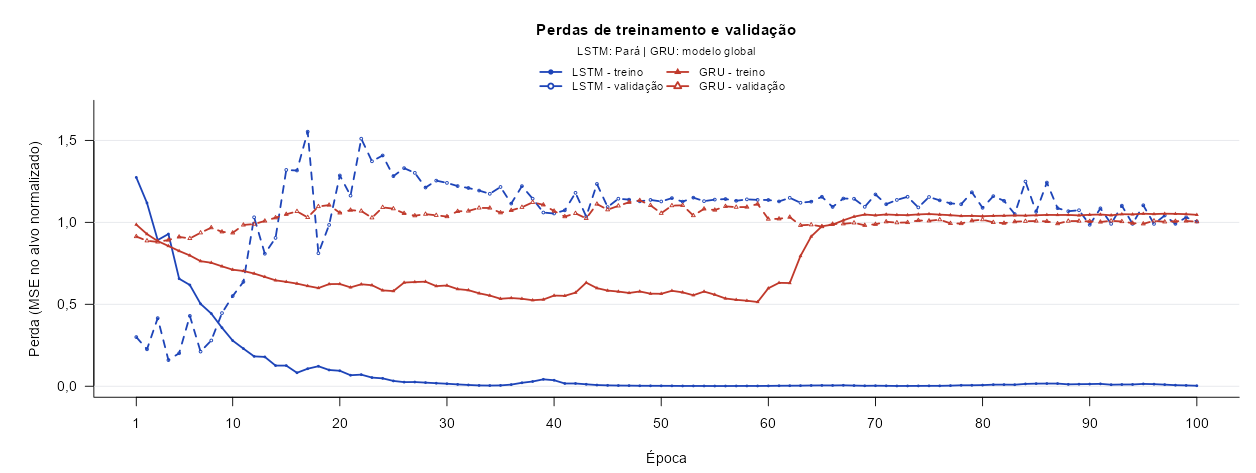
\includegraphics[width=\textwidth,height=1.2\textheight,keepaspectratio]{LSTMxGRUperdas.png}
        \caption{Projeção dos algoritmos LSTM e GRU 2025-2031.}
    \end{figure}
% \begin{itemize}
%    \item Curvas de perda e validação divergindo indicam Falta de capacidade de generalização dos algoritmos.
% \end{itemize}
 
\end{frame}

\begin{frame}{Sistema de Emissão de Relatório Parametrizado }

    \begin{figure}[H]
        \centering
        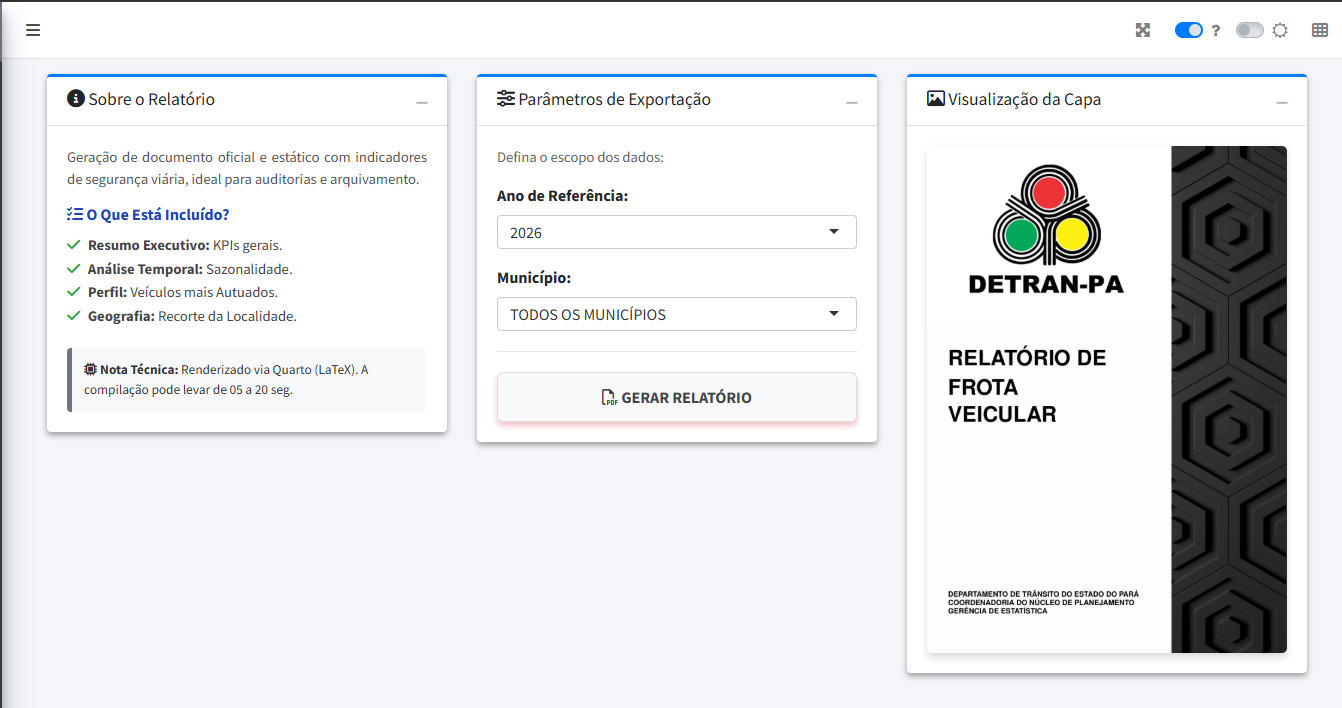
\includegraphics[width=\textwidth,height=0.8\textheight,keepaspectratio]{relatorio.png}
        \caption{Tela de Emissão do Relatório}
    \end{figure}
 \begin{itemize}
    \item O relatório é emitido de acordo com os parâmetros de município e ano escolhidos
 \end{itemize}
 
\end{frame}

\section{Sistema de Relatório Parametrizado}

\begin{frame}{Pipeline do Relatório Parametrizado}
    \begin{figure}[H]
        \centering
        \resizebox{0.95\textwidth}{!}{%
        \begin{tikzpicture}[
            node distance=0.8cm and 0.9cm,
            box/.style={draw, rectangle, rounded corners=4pt,
                minimum width=2.8cm, minimum height=1.8cm,
                align=center, font=\small},
            arrow/.style={-Stealth, thick, color=black!80}
        ]
        \node[box, fill=blue!10, draw=blue!40] (parametros)
            {\textbf{Parâmetros no Shiny}\\[6pt]
             \footnotesize Município\\
             \footnotesize Ano inicial};

        \node[box, right=of parametros,
            fill=green!10, draw=green!50] (quarto)
            {\textbf{Modelo Quarto}\\[6pt]
             \footnotesize \texttt{QUARTO\_DOC.qmd}\\
             \footnotesize Cópia temporária};

        \node[box, right=of quarto,
            fill=orange!10, draw=orange!50] (analise)
            {\textbf{Processamento em R}\\[6pt]
             \footnotesize Filtros com Arrow\\
             \footnotesize Gráficos: \texttt{ggplot2}\\
             \footnotesize Tabelas: \texttt{gt}};

        \node[box, right=of analise,
            fill=red!10, draw=red!40] (pdf)
            {\textbf{PDF Institucional}\\[6pt]
             \footnotesize LaTeX / TinyTeX\\
             \footnotesize \texttt{HEADER.tex}\\
             \footnotesize Download no Shiny};

        \node[box, above=of analise, minimum height=0.9cm,
            fill=gray!10, draw=gray!50] (dados)
            {\textbf{Base de Dados}\\
             \footnotesize \texttt{FROTA.parquet}};

        \draw[arrow] (parametros) --
            node[above, font=\scriptsize] {\texttt{params}} (quarto);
        \draw[arrow] (quarto) --
            node[above, font=\scriptsize] {Executa} (analise);
        \draw[arrow] (dados) --
            node[right, font=\scriptsize] {Consulta} (analise);
        \draw[arrow] (analise) --
            node[above, font=\scriptsize] {Compila} (pdf);
        \end{tikzpicture}%
        }
        \caption{Geração do boletim a partir do recorte territorial
        e temporal selecionado.}
    \end{figure}

    \vspace{0.15cm}
    \small
    \begin{itemize}
        \item \textbf{Preparação:} O módulo copia o modelo e os recursos
        visuais para uma pasta temporária antes da renderização.
        \item \textbf{Entrega:} O Shiny disponibiliza o PDF com nome
        definido pelo município e pelo ano selecionados.
    \end{itemize}
\end{frame}

\begin{frame}{Integração Contínua e DevOps}
    \begin{figure}[H]
        \centering
        \resizebox{0.8\textwidth}{!}{%
        \begin{tikzpicture}[
            node distance=0.8cm and 1.8cm,
            box/.style={draw, rounded corners = 3pt, rectangle, minimum width=2.8cm, minimum height=1.2cm, align=center, font=\footnotesize},
            db/.style={draw, cylinder, shape border rotate=90, aspect=0.25, minimum width=2.8cm, minimum height=1.2cm, align=center, font=\footnotesize},
            arrow/.style={-Stealth, thick}, 
            barrow/.style={Stealth-Stealth, thick}
        ]
        %% 1. NÓS INTERNOS
        \node[box] (scripts) {\Large\faRProject \\[4pt] ~ \texttt{(App.R)}};
        \node[box, below=of scripts] (docker) {\Large\faDocker \\[4pt]~ \texttt{(Dockerfile)}};
        \node[box, right=3.5cm of scripts] (repo) {\Large\faCodeBranch \\[4pt] Repositório};
        \node[db, below=1.2cm of repo] (registry) {\Large\faCubes \\[4pt] Container Registry};

        %% 2. CAIXAS TRACEJADAS
        \begin{scope}[on background layer]
            \node[box, dashed, inner sep=0.3cm, fit=(scripts)(docker), label={[font=\footnotesize]above: Ambiente Local}] (local) {};
            \node[box, dashed, inner sep=0.3cm, fit=(repo)(registry), label={[font=\footnotesize]above:GitLab}] (gitlab) {};
        \end{scope}

        %% 3. NÓS DE INFRAESTRUTURA
        \node[box, below=1cm of local] (podman) {\Large\faBox\\[4pt] Podman Build};
        \node[box, right=3.2cm of repo] (k8s) {\Large\faNetworkWired\\[4pt] Kubernetes};
        \node[box] at (k8s |- registry) (site) {\Large\faGlobe \\[4pt] Portal Web};
        \node[box, below=1.2cm of site] (cliente) {\Large\faDesktop \\[4pt] Usuário Final};

        %% 4. CONEXÕES
        \draw[arrow] (local.east |- repo.west) -- node[above, font=\scriptsize] {push} (repo.west);
        \draw[arrow] (local.south) -- (podman.north);
        \draw[arrow] (podman.east) -- node[above, sloped, font=\scriptsize] {push} (registry.west);
        \draw[arrow] (gitlab.east |- k8s.west) -- node[above, font=\scriptsize] {CI/CD} (k8s.west);
        \draw[arrow] (k8s.south) -- node[right, font=\scriptsize] {Expõe IP} (site.north);
        \draw[barrow] (site.south) -- node[left, font=\scriptsize] {WSS Segura} (cliente.north);
        \end{tikzpicture}%
        }
        \caption{Afinidade de sessão (\textit{sticky sessions}) configurada no Kubernetes para evitar perda de estado no Shiny.}
    \end{figure}
\end{frame}

\section{Pipeline CI/CD}

\begin{frame}{Deployment e CI/CD}
    \small
    \begin{block}{Implantação realizada}
        O \textbf{Podman} cria a imagem a partir do \texttt{Dockerfile},
        com R/Shiny e Quarto/TinyTeX. O \textbf{GitLab CI/CD} automatiza
        testes e publica a imagem no \textit{Container Registry}.
        O \textbf{Kubernetes} executa e gerencia as réplicas em pods.
    \end{block}

    \vspace{0.15cm}
    \textbf{Dificuldades com R Shiny e Kubernetes:}
    \begin{itemize}
        \item \textbf{Perda de estado:} O Shiny mantém o estado no processo R
        e usa WebSockets. Requisições enviadas a outro pod podem perder
        o acesso a esse estado.

        \item \textbf{Solução adotada:} Afinidade por cookies
        (\textit{sticky sessions}) no \textit{Ingress Controller}
        mantém as requisições de cada sessão no mesmo pod.

        \item \textbf{Limite de escalabilidade:} Adicionar réplicas não
        migra o estado das sessões ativas, podendo manter uma
        distribuição desigual de carga entre os pods.
    \end{itemize}

    \vspace{0.1cm}
    \begin{block}{Trabalho futuro}
        Investigar o \textbf{ShinyProxy} para gerenciar aplicações em
        contêineres e avaliar seu efeito com testes de carga.
    \end{block}
\end{frame}

% ==========================================
% SEÇÃO 5: CONCLUSÃO
% ==========================================
\section{Considerações Finais}

\begin{frame}{Considerações Finais e Trabalhos Futuros}
    \begin{itemize}
        \item \textbf{Solução Implementada:} Arquitetura orquestrada (R, Shiny, Apache Arrow, Kubernetes) elimina limitações de BI proprietário e consolida a Transparência Ativa governamental.
        \item \textbf{Impacto Preditivo:} Modelos robustos apontam um limite logístico alarmante: crescimento acelerado com projeção de saturação na infraestrutura das rodovias (acréscimo de 60 mil veículos anuais até 2031).
        \item \textbf{Dataset mais detalhado:} Para a implementação de algoritmos de Deep Learning é necessário um dataset mais robusto e mais extensivo (dias como amostra em vez de meses).
        \item \textbf{Inteligência Institucional:} A previsão de malha veicular baliza diretamente o planejamento fazendário (IPVA e Licenciamentos) e as ações da secretaria de transporte.
        \item \textbf{Próximos Passos:} Migrar a infraestrutura relacional estática para processamento em tempo real de acidentes e infrações via \textit{Apache Kafka} (\textit{Stream Processing}).
    \end{itemize}
\end{frame}

% --- SLIDE FINAL ---
\begin{frame}
    \centering
    \Huge \textbf{Muito Obrigado!}
    \vspace{1cm}
    
    \Huge \textbf{THANKS}
    \vspace{1cm}
    \\
    \large \textbf{Gabriel Baia da Silva} \\
    \normalsize \texttt{gabriel.baia@detran.pa.gov.br}
    
    \vspace{0.5cm}
    \normalsize Mário Diego Rocha Valente \\
    \normalsize Kleber Bezerra Salim \\
    \normalsize Tito Félix de Oliveira
\end{frame}

\end{document} 